\section{Grain growth opacity and radiative windows} \label{radwindow}

The opacity of the interstellar medium is reasonably well constrained and approximate analytic expressions for the Rosseland mean opacity as a function of temperature and density are derived in \citet{bell94}. For low temperatures ($T \lesssim 100$ K) at which ice grains are present, opacity scales with temperature as $\kappa \sim T^2$. Sublimation of ice grains at $\sim$$150$ K and of metal grains at $\sim$$1000$ K results in sharp opacity drops. This is shown in Figure \ref{fig:opacity} for a gas density $\rho=10^{-8}$ g cm$^{-3}$, which is typical for the outer regions of protoplanetary disks. \citet{semenov03} calculate Rosseland mean opacities in protoplanetary disks for grains of different sizes and structure. As shown in Figure \ref{fig:opacity}, their results are in good agreement with \citet{bell94}. However, \citet{semenov03} do not take grain growth into account, which is likely to occur in protoplanetary disks, particularly at the late times when cores form. \citet{dalessio01} compute wavelength dependent opacities for a range of maximum particle sizes and different size distributions. Figure \ref{fig:opacity} shows the integrated Rosseland mean opacity for a maximum particle size of 1 cm and a power law differential size distribution $dN/ds \propto s^{-p}$, with $s$ the grain size and $p=3.5$ for a standard collisional cascade and $p=2.5$ when coagulation is taken into account. We see in Figure \ref{fig:opacity} that this yields a mean opacity that is both lower and less sensitive to temperature, when compared to \citet{bell94} or \citet{semenov03}. However, \citet{dalessio01} only computes opacities for temperatures less than the dust sublimation temperature, appropriate for current observations of dust in protoplanetary disks. As we see in Figure \ref{fig:opacity}, the opacity dramatically decreases during dust sublimation. We thus use the \citet{bell94} opacities for $T \gtrsim 1000$ K, ensuring that they smoothly match the \citet{dalessio01} opacities for lower temperatures.

\begin{figure}[h!]
\centering
%\includegraphics[width=0.5\textwidth]{../../figs/ModelAtmospheres/RadSelfGravRealEOS/PaperFigs/kappa_grain_growth_SBL_paper.pdf}
\includegraphics[width=0.5\textwidth]{figures/kappa_grain_growth_SBL_paper.pdf}
%%\vspace{-0.5in}
\caption{Rosseland mean opacity of dust grains as a function of temperature for different opacity assumptions. The dashed black curve shows the \citet{bell94} analytic ISM opacity for $\rho=10^{-8}$ g cm$^{-3}$. The solid black curve shows the tabulated opacity of \citet{semenov03} for a dust composition of 'normal' silicates. The dashed red curve shows the \citet{dalessio01} opacity, which takes grain growth into account, for a maximum particle size of 1 cm and a standard collisional cascade grain size distribution ($p=3.5$). The solid red curve is the same as the dashed red curve, but it accounts for coagulation ($p=2.5$).}
\label{fig:opacity}
\end{figure}

The significant opacity drop due to the sublimation of ice and metal grains lowers the radiative temperature gradient $\delrad$, which may result in one or more inner radiative layers inside the atmosphere of a protoplanet. This is displayed in Figure \ref{fig:delvsr}: depending on the semimajor axis and core mass, the opacity drop will generate no radiative window (top panel), one radiative window (middle panel), or two radiative windows (bottom panel). 

\begin{figure}[h!]
\centering
%\includegraphics[width=0.5\textwidth]{../../figs/ModelAtmospheres/RadSelfGravRealEOS/PaperFigs/del_vs_r.pdf}
\includegraphics[width=0.5\textwidth]{figures/del_vs_r.pdf}
%%\vspace{-0.5in}
\caption{Snapshots of the radiative and adiabatic gradient as a function of the radial coordinate, for planets with different core masses forming at various locations in the disk. The nebular gas is described by a realistic EOS, with a standard collisional cascade size distribution ($p=3.5$). The sharp drop in opacity due to dust sublimation may generate one or more radiative windows. Top panel: no radiative window for $a=100$ AU and $M\co=3 M_{\oplus}$. Middle panel: the sharp opacity decrease produces one radiative window for $a=50$ AU and $M\co=5 M_{\oplus}$. Bottom panel: the decrease in opacity results in two radiative windows for $a=20$ AU and $M\co=3 M_{\oplus}$.}
\label{fig:delvsr}
\end{figure}


%This is not a problem, however, if most atmospheric luminosity is generated in the innermost convective region of the envelope (see \S\ref{sec:opacity}). We can check this \textit{a posteriori} by using the local energy equation,
%\begin{equation}
%\label{eq:localen}
%\frac{\partial L}{\partial m}=-T \frac{\partial S}{\partial t},
%\end{equation}
%assuming that $\partial S/\partial t$ is constant for a given atmospheric profile. Our model is then valid if $\Delta I \ll I$, where
%\begin{equation}
%\label{eq:I}
%I = \int_{M_{\rm c}}^{M_{\rm{RCB_1}}} T d m
%\end{equation}
%and
%\begin{equation}
%\label{eq:I}
%\Delta I = \int_{M_{\rm{RCB_1}}}^{M_{\rm p}}T d m,
%\end{equation}
%with $\rm{RCB_1}$ the innermost RCB and $M_{\rm p}$ the total planet mass. We find $\Delta I /I \lesssim 30\%$ for all our models of interest (see, however, \S\ref{sec:opacity} and \S\ref{critical} for exceptions). 

%\textit{Radiative windows could, in principle, change atmospheric structure and thus affect evolution if most luminosity is not generated in the innermost convective region of the envelope. } 

{Our idealization of a constant $L$ with radius may be challenged by the presence of radiative windows. While the structure of convective regions is unaffected by $L$, the structure of radiative windows depends on $L$. Fortunately, the assumption of constant luminosity remains reasonable if most of the luminosity is generated in the innermost convective region of the envelope. We can check whether this is true \textit{a posteriori} by using the local energy equation,
\begin{equation}
\label{eq:localen}
\frac{\partial L}{\partial m}=-T \frac{\partial S}{\partial t},
\end{equation}
and integrating it between $M\co$ and $M_{\rm{RCB_1}}$, where $\rm{RCB_1}$ is the innermost RCB. This luminosity can be as little as half of the assumed fixed atmospheric luminosity $L$.

Self-consistently calculating $L(r)$ is not feasible for our code. Instead, we note that since  $\partial S/\partial t$ is fixed in convective regions \citep{arras06}, the luminosity profile is more centrally concentrated than $L \propto m$, which can be implemented simply.  We calculated example profiles using $L \propto m$ and found that though this luminosity scaling may move the location of the outermost RCB, it does not substantially change the luminosity emerging at the top of the atmosphere or the time evolution. %This result may be understood by noting that small changes in the relative normalization of $\delad$ and $\delrad$ in Figure \ref{fig:delvsr} can change the location of the RCB without affecting structure significantly.

%We therefore expect our results to approximate those for the true $L(r)$.

%assuming that $\partial S/\partial t$ is constant for a given atmospheric profile. Our model is then valid if $\Delta I \ll I$, where
%\begin{equation}
%\label{eq:I}
%I = \int_{M_{\rm c}}^{M_{\rm{RCB_1}}} T d m
%\end{equation}
%and
%\begin{equation}
%\label{eq:I}
%\Delta I = \int_{M_{\rm{RCB_1}}}^{M_{\rm p}}T d m,
%\end{equation}
%with $\rm{RCB_1}$ the innermost RCB and $M_{\rm p}$ the total planet mass. We find $\Delta I /I \lesssim 30\%$ for all our models of interest (see, however, \S\ref{sec:opacity} and \S\ref{critical} for exceptions). 

%If radiative windows exist, our model requires most of the atmospheric luminosity to be generated in the innermost convective region. By design, the luminosity in the radiative windows, $L_{\rm radw}$, must satisfy $L_{\rm radw}=L$, where $L$ is the assumed fixed luminosity at the top of the atmosphere. Non-negligible extra luminosity generated in the outer convective layers would, however, yield $L_{\rm radw}<L$, in conflict with our assumptions, and could change atmospheric structure. A simple way to check this \textit{a posteriori} is by rewriting the local energy equation (\ref{eq:structd}) as $\partial L/\partial m=-T \partial S/\partial t$, and integrating it throughout the atmosphere assuming that $\partial S/\partial t$ is fixed (e.g., \citealt{arras06}). If the value of this integral, $I$\footnote{This integral does not have units of luminosity, as we drop the constant $\partial S/\partial t$ term.}, throughout the innermost convective region is significantly larger than its value throughout the rest of the envelope, $\Delta I$, then our assumptions hold. For all the models for which $\Delta L \ll L$ holds (see paragraph above), we have found $\Delta I / I \lesssim 30\%$, and typically $\lesssim 10\%$ (see \App{radwindow} for additional details).

%A more rigorous check would be comparing our models with constant $L$ throughout with example profiles for which $L \propto \int T dm$. In practice, this calculation is not feasible for our code. However, we can make a simple estimate of how a non-constant $L$ affects atmospheric structure by assuming $L \propto m$ throughout the atmosphere. Note that $L \propto \int T dm$ makes the luminosity more centrally concentrated than if $L \propto m$, so our simple estimate is conservative. We have found that $L \propto m$ may change atmospheric structure by moving the outermost RCB closer to the top of the envelope, but this does not change the atmospheric luminosity or time evolution.

%As an additional check that the atmospheric structure and evolution are not changed due to the radiative windows, we 

